\documentclass{article}
\usepackage[utf8]{inputenc}
\usepackage{mathtools, amssymb, amsthm}
\usepackage{fullpage}
\usepackage{physics}
\usepackage{siunitx}
\usepackage{comment}

\usepackage{tikz}
\usetikzlibrary{arrows}

\usepackage[
    pdfusetitle,
    colorlinks
]{hyperref}

\title{Modeling and simulation of the SLM process}
\date{\today}
\author{Oleg Rogozin}

\newcommand{\dder}[2][]{\Delta_{#2}#1}
\newcommand{\diag}[1]{\qty(#1)^\mathrm{diag}}
\newcommand{\fusion}[1]{{#1}^\mathrm{fus}}

% dimensionless variables
\newcommand{\Hx}{\hat{x}}
\newcommand{\Ht}{\hat{t}}
\newcommand{\Hh}{\hat{h}}
\newcommand{\HT}{\hat{T}}
\newcommand{\HP}{\hat{P}}
\newcommand{\Halpha}{\hat{\alpha}}
\newcommand{\Hsigma}{\hat{\sigma}}
\newcommand{\Hf}{\hat{f}}
\newcommand{\Hc}{\hat{c}}
\newcommand{\Hk}{\hat{k}}
\newcommand{\Hphi}{\hat{\phi}}
\newcommand{\Hpsi}{\hat{\psi}}

\begin{document}
\maketitle
\tableofcontents

\section{Formulation of the problem}

%%% The first law of thermodynamics
The conservation of energy for a substance at rest is described by the \(D\)-dimensional heat-conduction equation
\begin{equation}\label{eq:heat_conduction}
	\rho\pdv{h(T)}{t} = \pdv{x_i}\qty( k(\psi,T)\pdv{T}{x_i} ),
\end{equation}
where \(x_i\) are the physical coordinates (\si{m}), \(t\) is the time (\si{s}),
\(\rho\) is the density (\si{kg/m}\(^D\)), \(h\) is the specific enthalpy (\si{J/kg}),
\(T\) is the temperature (\si{\K}), \(k\) is the thermal conductivity (\si{W/Km}\(^{D-2}\)),
\(\psi\) is the porosity. Let
\begin{equation}\label{eq:porosity_variables}
	\rho = \rho_0(1-\psi_0), \quad k = k_0(T)(1-\psi),
\end{equation}
where \(\rho_0\) and \(k_0\) is the density and thermal conductivity of the bulk material, respectively,
\(\psi_0\) is the initial porosity.

%%% Introduce a liquid fraction
To incorporate the fusion process into the model, let the enthalpy depends on the temperature as follows:
\begin{equation}\label{eq:enthalpy}
	h = \int_{T_0}^T c_p(\xi)\dd{\xi} + \fusion{h}\phi(h),
\end{equation}
where \(c_p\) is the specific heat capacity (\si{J/kgK}), \(\fusion{h}\) is the specific enthalpy of fusion (\si{J/kg}),
\(\phi\) is the liquid fraction (\(0 \leq \phi \leq 1\)).
\(\phi=0\) and \(\phi=1\) corresponds to the solid and liquid states, respectively.
Substituting~\eqref{eq:porosity_variables} and~\eqref{eq:enthalpy} into~\eqref{eq:heat_conduction}, we obtain
\begin{equation}\label{eq:heat_conduction2}
	\rho_0\pdv{h}{t} = \pdv{x_i}\qty( \frac{1-\psi}{1-\psi_0} \frac{k_0(T)}{c_p(T)}\pdv{h_*}{x_i} ),
\end{equation}
where \(h_* = h - \fusion{h}\phi\) is introduced for convenience.

%%% Change in thermophysical properties resulting from fusion process
The phase transition results in an abrupt change in the thermophysical properties \(f=c_p,k_0\) of the material;
therefore, they can be expressed as
\begin{equation}\label{eq:fusion_change}
	f = f_S(T) + \qty( f_L(T) - f_S(T) )\phi,
\end{equation}
where \(f_S\) and \(f_L\) correspond to solid and liquid properties.
The porosity change is irreversible in time:
\begin{equation}\label{eq:porosity}
	\psi(t) = \psi_0\min_{0\leq\tau\leq t}\qty( 1-\phi(h(\tau)) ).
\end{equation}

%%% Initial and boundary conditions
Consider a half-space problem \(x_D<0\) with the following boundary condition at \(x_D=0\):
\begin{equation}\label{eq:bc}
	k(\psi,T)\pdv{T}{x_D} = \frac{A(\psi)P}{(\pi R^2)^{(D-1)/2}}\exp\qty( -\frac{(x_i-x_{Bi}(t))^2}{R^2} )
	    - \alpha(T-T_0) - \epsilon\sigma T^{D+1},
\end{equation}
where \(A\) is the absorptivity, \(P\) is the laser power (\si{W}), \(R\) is the radius of the laser beam (\si{m}),
\(x_{Bi}\) are the coordinates of its center (\si{m}), \(\alpha\) is the convective heat transfer coefficient (\si{W/Km}\(^{D-1}\)),
\(\epsilon\) is the emissivity, \(\sigma\) is the Stefan--Boltzmann constant (\si{W/K}\(^{D+1}\)\si{m}\(^{D-1}\)).
The initial condition is \(T=T_0\) at \(t=0\).

\subsection{Dimensionless expressions}

Introduce the following dimensionless variables:
\begin{equation}\label{eq:dimensionless}
    \begin{aligned}
        x_i &= \Hx_iR, & t &= \Ht t_0, & h &= \Hh c_p(T_0)\Delta{T}, & T - T_0 &= \HT\Delta{T}, \\
        P &= \HP k_0(T_0)\Delta{T}R^{D-2}, & \alpha &= \Halpha\frac{k_0(T_0)}R, &
            \sigma &= \Hsigma\frac{k_0(T_0)}{R\Delta{T}^D}, & T_0 &= \HT_0\Delta{T}, \\
    \end{aligned}
\end{equation}
where \(t_0 = \rho_0 c_p(T_0) R^2/k_0(T_0)\) is the diffusive time scale at \(T=T_0\),
\(\Delta{T} = (T_S+T_L)/2 - T_0\) is the unit temperature,
\(T_S\) and \(T_L\) are the solidus and liquidus temperatures, respectively.
If \(|\pdv*{x_{Bi}}{t}|\) is of order \(U_0\), where \(U_0\) is the reference scanning speed (\si{m/s}),
then \(R/U_0\) is the convective time scale. Also denote
\begin{equation}\label{eq:dimensionless2}
    \Hc_p(\HT) = \frac{c_p(T)}{c_p(T_0)}, \quad
    \Hk_0(\HT) = \frac{k_0(T)}{k_0(T_0)}, \quad
    \Hphi(\Hh) = \phi(h), \quad
    \Hpsi(\Hh) = \psi(h).
\end{equation}
Then~\eqref{eq:enthalpy},~\eqref{eq:heat_conduction2}, and~\eqref{eq:bc} take the following nondimensional form:
\begin{gather}
	\Hh_* \equiv \Hh - \fusion{\Hh}\Hphi = \int_0^{\HT} \Hc_p(\xi)\dd{\xi}, \label{eq:enthalpy_hats} \\
	\pdv{\Hh}{\Ht} = \pdv{\Hx_i}\qty(
	    \frac{1-\Hpsi}{1-\psi_0}
	    \frac{\Hk_0(\HT)}{\Hc_p(\HT)}\pdv{\Hh_*}{\Hx_i}
	), \label{eq:heat_conduction_hats} \\
	\qty(1 - \Hpsi) \frac{\Hk_0(\HT)}{\Hc_p(\HT)}\pdv{\Hh_*}{\Hx_D} +
	    \Halpha\HT + \epsilon\Hsigma \qty(\HT + \HT_0)^{D+1} =
	    \frac{A(\Hpsi)\HP}{\pi^{(D-1)/2}}\exp\qty( -\qty(\Hx_i-\Hx_{Bi}(t))^2 ). \label{eq:bc_hats}
\end{gather}
The initial condition is \(\Hh = 0\).

\subsection{Thermophysical properties}

For conventional materials, the required thermophysical properties can be reasonably approximated
by the three-parameter model (Fig.~\ref{fig:thermophysical})
\begin{equation}\label{eq:thermophysical_model}
	\Hf = 1 + \Hf'_S\HT + \qty[
	    \fusion{\Hf} + \qty(\Hf'_L-\Hf'_S) \qty(\HT-1)
	]\Hphi,
\end{equation}
where \(\Hf'_{S,L}\) are the corresponding constant first temperature derivatives far from fusion process,
\(\fusion{\Hf}\) is the property jump at the phase transition.
Matching~\eqref{eq:thermophysical_model} with~\eqref{eq:fusion_change}, we obtain
\begin{equation}\label{eq:thermophysical_model_explicit}
	\Hf_S = 1 + \Hf'_S\HT, \quad
	\Hf_L = \Hf_{L0} + \Hf'_L\HT,
\end{equation}
where \(\Hf_{L0} = 1 + \Hf'_S - \Hf'_L + \fusion{\Hf}\).

\begin{figure}
    \centering
    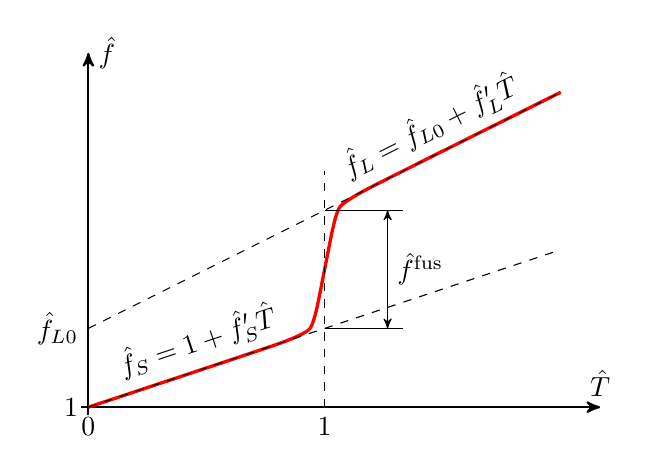
\begin{tikzpicture}[thick, >=stealth']
        \coordinate (O) at (0,0);
        \draw[->] (-0.1,0) -- (6.5,0) node[above] {$\HT$} coordinate(xmax);
        \draw[->] (0,-0.1) -- (0,4.5) node[right] {$\Hf$} coordinate(ymax);

        \path (O) -- (3,1) node[midway,sloped,above] {$\Hf_S=1+\Hf'_S\HT$}
            -- (3,2.5) -- (6,4) node[midway,sloped,above] {$\Hf_L=\Hf_{L0}+\Hf'_L\HT$};
        \draw[red, very thick] plot[smooth,tension=0.3,mark=] coordinates{
            (0,0) (2.4,2.4/3) (2.8, 2.8/3+0.05) (2.9,3.5/2-0.5) (3.1,3.5/2+0.5) (3.2,2.5+0.2/2-0.05) (3.6,2.5+0.6/2) (6,4)};
        \draw[thin,dashed] (0,1) coordinate(A) -- (6,4);
        \draw[thin,dashed] (O) -- (6,2);
        \draw[thin,dashed] (3,0) coordinate(F) -- (3,3);

        \node[below] at (O) {$0$};
        \node[below] at (F) {$1$};
        \node[left] at (O) {$1$};
        \node[left] at (A) {$\Hf_{L0}$};

        \draw[thin] (3,1) -- (4,1);
        \draw[thin] (3,2.5) -- (4,2.5);
        \draw[thin,<->] (3.8,1) -- (3.8,2.5) node[midway,right] {$\fusion{\Hf}$};
    \end{tikzpicture}
    \caption{Dimensionless thermophysical properties versus temperature for the three-parameter model~\eqref{eq:thermophysical_model}.}
    \label{fig:thermophysical}
\end{figure}

\section{Liquid fraction models}

Impose the following physical requirements upon \(\hat\phi(\Hh)\):
\begin{gather}
    0 \leq \dv{\hat\phi}{\Hh} \leq \eval{\dv{\hat\phi}{\Hh}}_{\Hh=\Hh(1)} =
        \frac1{\Hh(\HT_L)-\Hh(\HT_S)}, \label{eq:lf_monotonic}\\
    \hat\phi\qty(\Hh(1) - \Hh) = 1 - \hat\phi(\Hh) \quad \qty(\Hh\geq\Hh(1)), \label{eq:lf_symmetric}\\
    \begin{cases}
	\phi(\Hh) = \order{(\Hh(\HT_S)-\Hh)^{-\infty}} \quad \qty(\Hh < \Hh(\HT_S)), \\
	    \phi(\Hh) = \order{(\Hh-\Hh(\HT_L))^{-\infty}} \quad \qty(\Hh > \Hh(\HT_L)).
	\end{cases}\label{eq:lf_exp_decay}
\end{gather}
Inequalities~\eqref{eq:lf_monotonic} are the monotonic condition and boundedness of the fusion rate,
\eqref{eq:lf_symmetric} is the symmetric property,
and~\eqref{eq:lf_exp_decay} describes an exponential decay of \(\hat\phi(\Hh)\) outside the fusion range.

The simplest \(\mathcal{C}^0\) model for \(\Hphi(\Hh)\) can be constructed as a piecewise approximation
\begin{equation}\label{eq:lf_piecewise}
	\Hphi = \begin{cases}
        0,                                            & \Hh \leq \Hh(\HT_S), \\
        \frac{\Hh-\Hh(\HT_S)}{\Hh(\HT_L)-\Hh(\HT_S)}, & \Hh(\HT_S) < \Hh < \Hh(\HT_L), \\
        1,                                            & \Hh(\HT_L) \leq \Hh.
    \end{cases}
\end{equation}
Except \(\fusion{\Hh}\), \(\delta\fusion{\HT} = \HT_L - \HT_S\)
is the only parameter of the fusion process  used in~\eqref{eq:lf_piecewise}.
Employing cubic splines near \(h_S\) and \(h_L\) yields the more realistic two-parameter \(\mathcal{C}^1\) model:
\begin{equation}\label{eq:lf_splines}
	\dots
\end{equation}

\section{Temperature evaluation}

For arbitrary \(\Hphi(\Hh)\), solution of~\eqref{eq:enthalpy_hats} is not straightforward.
However, the temperature is included in~\eqref{eq:heat_conduction_hats} only through thermophysical properties
and, therefore, can be evaluated quite roughly.
Direct dependence of boundary conditions~\eqref{eq:bc_hats} on temperature is also weak.
Several approaches can be proposed to find a simplified approximation of \(\HT(\Hh)\).

\subsection{\(\mathcal{C}^1\) approximation}

\begin{table}[ht]
    \centering
    \caption{Piecewise quantities for~\eqref{eq:temp_crude}}
    \label{table:temp_params}
    \begin{tabular}{c|cccc}
        \hline\\[-1em]
        \(\Hh\)                           & \(\Hc'_p\)    & \(\Hc_{p0}\)  & \(\HT^\dag\) & \(\Hh^\dag\) \\[0.3em]
        \hline\\[-1em]
        \(\Hh \leq \Hh(\HT_S)\)           & \(\Hc'_{pS}\) & \(1\)         & \(0\)        & \(0\)        \\[0.3em]
        \(\Hh(\HT_S) < \Hh < \Hh(\HT_L)\) & \(a\)         & \(b\)         & \(\HT_S\)    & \(\Hh_1\)    \\[0.3em]
        \(\Hh(\HT_L) \leq \Hh\)           & \(\Hc'_{pL}\) & \(\Hc_{pL0}\) & \(\HT_L\)    & \(\Hh_2\)    \\[0.3em]
        \hline
    \end{tabular}
\end{table}

An acceptable accuracy can be achieved if the heat capacity is assumed
to depend on temperature linearly during a fusion process, i.e.,
\begin{equation}\label{eq:cp_crude}
	\Hc_p = \begin{cases}
        1 + \Hc'_{pS}\HT,         & \quad \Hh \leq \Hh(\HT_S), \\
        b + a\HT,                 & \quad \Hh(\HT_S) < \Hh < \Hh(\HT_L), \\
        \Hc_{pL0} + \Hc'_{pL}\HT, & \quad \Hh(\HT_L) \leq \Hh,
    \end{cases}
\end{equation}
where
\begin{equation*}
	\Hc_{pL0} = 1 + \fusion{\Hc_p} + \Hc'_{pS} - \Hc'_{pL}, \quad
	a = \frac{\Hc'_{pS} + \Hc'_{pL}}2 + \frac{\fusion{\Hc_p}}{\delta\fusion{\HT}}, \quad
	b = 1 + \HT_S\qty(\Hc'_{pS} - a).
\end{equation*}
Substituting~\eqref{eq:cp_crude} into~\eqref{eq:enthalpy_hats},
we obtain that the temperature is calculated as a root of the quadratic equation
\begin{equation}\label{eq:temp_crude}
	\HT = \HT^\dag + \frac{\sqrt{\Hc_{p0}^2 + 2\Hc_p'(\Hh_* - \Hh^\dag) } - \Hc_{p0}}{\Hc'_p},
\end{equation}
with the piecewise quantities defined in Tab.~\ref{table:temp_params}. Finally,
\begin{equation}\label{eq:enthalpySL_crude}
	\Hh(\HT_S) = \fusion{\Hh}\Hphi_S + \Hh_1, \quad \Hh(\HT_L) = \fusion{\Hh}\Hphi_L + \Hh_1 + \Hh_2,
\end{equation}
where \(\Hphi_{S,L} = \Hphi(\Hh(\HT_{S,L}))\) and
\begin{equation*}
	\Hh_1 = \HT_S\qty(1 + \frac{\Hc'_{pS}}2\HT_S), \quad
	\Hh_2 = \delta\fusion{\HT}\qty(b + \frac{a}2\delta\fusion{\HT}).
\end{equation*}

%%% Smoothness of c_p
Note that \(\dd\Hc_p/\dd\Hh\in\mathcal{C}^1\)
only if \(\Hphi(\Hh)\in\mathcal{C}^1\) and \(\Hc_p\in\mathcal{C}^0\).
Therefore, using \(\mathcal{C}^1\) model~\eqref{eq:lf_splines} for calculating \(\Hc_p(\HT)\)
and \(\mathcal{C}^0\) model~\eqref{eq:cp_crude} for calculating \(\HT\)
ensure that \(\dd\Hc_p/\dd\Hh\in\mathcal{C}^1\).

%%% Simple case
If \(\Hc'_{pL} = \Hc'_{pS} = \Hc'_p\) and \(\fusion{\Hc_{p}} = 0\),
then~\eqref{eq:temp_crude} can be rewritten as
\begin{equation}\label{eq:temp_crude2}
	\HT = \frac{\sqrt{1+2\Hc_p'\Hh_*}-1}{\Hc_p'}
\end{equation}
when \(\Hc_p'>0\) and \(\HT = \Hh_*\) when \(\Hc_p'=0\).

\subsection{\(\hat\phi\)-based approximation}

Another way is to use~\eqref{eq:fusion_change} for \(f=h\) with the five-parameter model:
\begin{equation}\label{eq:enthalpy_phi}
	\Hh = \Hh'_S\HT + \frac{\Hh''_S}2\HT^2 + \qty[
	    \fusion{\Hh} + \qty(\Hh'_L-\Hh'_S) \qty(\HT-1) + \frac{\Hh''_L-\Hh''_S}2 \qty( \HT^2-1 )
	]\Hphi,
\end{equation}
where
\begin{equation}\label{eq:enthalpy_phi_params}
	\Hh'_S = 1, \quad \Hh'_L = 1 + \Hc'_{pS} - \Hc'_{pL} + \fusion{\Hc}_p, \quad
	\Hh''_S = \Hc'_{pS}, \quad \Hh''_L = \Hc'_{pL}
\end{equation}
should be fulfilled for~\eqref{eq:enthalpy_phi} to be consistent with \(\Hc_p(\HT)\)
defined as~\eqref{eq:thermophysical_model}.
Indeed,~\eqref{eq:enthalpy_phi_params} results from the following assumption:
\begin{equation}\label{eq:enthalpy_phi_explicit}
	\Hh_S(\HT) = \int_0^{\HT} \Hc_{pS}(\xi)\dd{\xi}, \quad
	\Hh_L(\HT) = \int_0^1 \Hc_{pS}(\xi)\dd{\xi} + \fusion{\Hh} + \int_1^{\HT} \Hc_{pL}(\xi)\dd{\xi},
\end{equation}
where \(\Hc_{pS,L}\) is defined as~\eqref{eq:thermophysical_model_explicit}.

Actually,~\eqref{eq:enthalpy_phi} is the quadratic equation with respect to \(\HT\), hence
\begin{equation}\label{eq:temp_phi}
	\HT = \frac{\sqrt{\Hh'^2 + 2\Hh''\Hh_*}-\Hh'}{\Hh''},
\end{equation}
where \(\Hh^{\prime,\prime\prime} = \Hh_S^{\prime,\prime\prime} (1-\hat\phi) + \Hh_L^{\prime,\prime\prime}\hat\phi\).

\section{Numerical methods}

\subsection{Perturbation and its diagonal part}

With~\eqref{eq:heat_conduction_hats},~\eqref{eq:thermophysical_model},~\eqref{eq:temp_phi},
and arbitrary \(\Hphi(\Hh)\), we can employ the following expressions for numerical simulation:
\begin{gather}
    F = \dder{\Hx_i}\qty(
        \frac{1 - \Hpsi}{1 - \psi_0} \frac{\Hk_0(\HT)}{\Hc_p(\HT)} \dder[\Hh_*]{\Hx_i}
	), \\
    \var{F} = \dder{\Hx_i}\qty[ \frac{1 - \Hpsi}{1 - \psi_0} \qty(
	    \dv{\Hh_*}(\frac{\Hk_0(\HT)}{\Hc_p(\HT)})\var{\Hh_*}\dder[\Hh_*]{\Hx_i} +
	    \frac{\Hk_0(\HT)}{\Hc_p(\HT)} \dder[\var{\Hh_*}]{\Hx_i}
	)], \\
    \diag{\var{F}} = \frac{1 - \Hpsi}{1 - \psi_0} \qty(
	    \dv{\Hh_*}(\frac{\Hk_0(\HT)}{\Hc_p(\HT)})\dder[\Hh_*]{\Hx_i} \diag{\dder{\Hx_i}} +
	    \frac{\Hk_0(\HT)}{\Hc_p(\HT)} \diag{\dder{\Hx_i}^2}
	)\diag{\var{\Hh_*}}.
\end{gather}
where
\begin{equation}
    \var{\Hh_*} = \qty(1 - \fusion{\Hh}\hat\phi')\var{\Hh}, \quad
    \diag{\Hh_*} = \diag{\var{\Hh_*}} = 1 - \fusion{\Hh}\hat\phi'(\Hh).
\end{equation}

\subsection{Boundary conditions}

Nonlinear dependence~\eqref{eq:temp_phi} can be linearized; therefore, we have the following linear boundary condition at \(\Hx_D=0\):
\begin{multline}\label{eq:bc_linearized}
	\qty[
	    \qty(1 - \Hpsi^n) \frac{\Hk_0(\HT^n)}{\Hc_p(\HT^n)} \qty(1-\fusion{\Hh}\hat\phi'(\Hh^n))\pdv{\Hx_D} +
	    \dv{\HT^n}{\Hh}\qty( \Halpha\HT^n + \epsilon\Hsigma(D+1) \qty(\HT^n + \HT_0)^D )
	]\Hh = \\ \frac{A(\Hpsi^n)\HP}{\pi^{(D-1)/2}}\exp\qty( -\qty(\Hx_i-\Hx_{Bi}^n)^2 ) -
        \Halpha\HT^n - \epsilon\Hsigma\qty(\HT^n + \HT_0)^{D+1}.
\end{multline}
where superscript \(n\) corresponds to values calculated at the previous time step.

\subsection{Liquid fraction models}

For the piecewise approximation~\eqref{eq:lf_piecewise},
\begin{equation}
	\fdv{\Hphi}{\Hh} = \diag{\var{\Hphi}} = \begin{cases}
        0 & \quad \Hh \leq \Hh(\HT_S), \quad \Hh(\HT_L) \leq \Hh, \\
        1/(\Hh(\HT_L)-\Hh(\HT_S)) & \quad \Hh(\HT_S) < \Hh < \Hh(\HT_L). \\
    \end{cases} \label{eq:pert_phi_h_diag}
\end{equation}

\end{document}

0 = T + c'T^2 + phi - h
T = (-1+\sqrt{1+4c'(h-phi)})/2c'
\psi = \psi_0 -- \phi=0
\psi = 0      -- \phi=1
\psi = \psi_0 - \phi\psi_0

